\section{Parcelando la corteza}

\subsection{Utilizando LogOdds}

\begin{figure}[h!]
                                                                                                                        
\begin{minipage}[b]{\textwidth}
    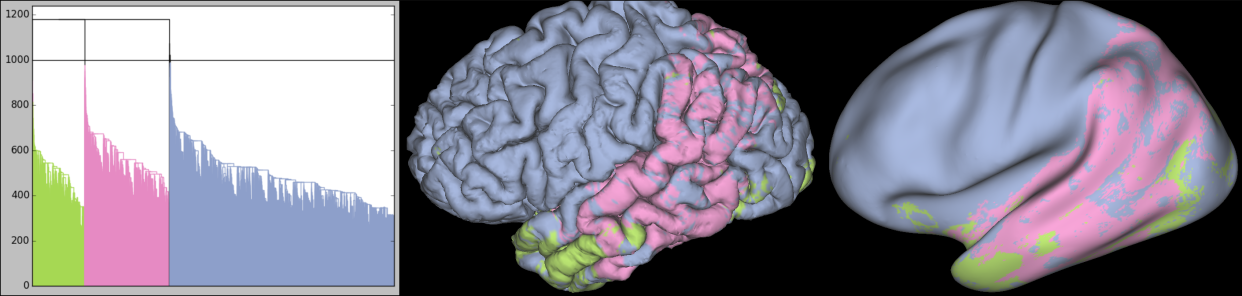
\includegraphics[width=\textwidth]{img/all_brain/logit_0.png}
    \caption{M\'etodo Logit sin preprocesamiento}
    \label{fig:dmri}
\end{minipage} ~
                                                                                                                        
\begin{minipage}[b]{\textwidth}
    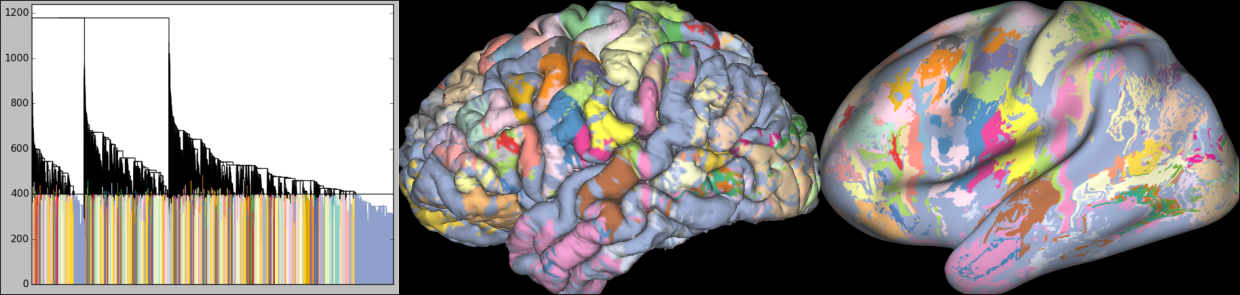
\includegraphics[width=\textwidth]{img/all_brain/logit_0_deep.png}
    \caption{M\'etodo Logit sin preprocesamiento, mayor profundidad en el 
            dendrograma}

\end{minipage} ~

\begin{minipage}[b]{\textwidth}
    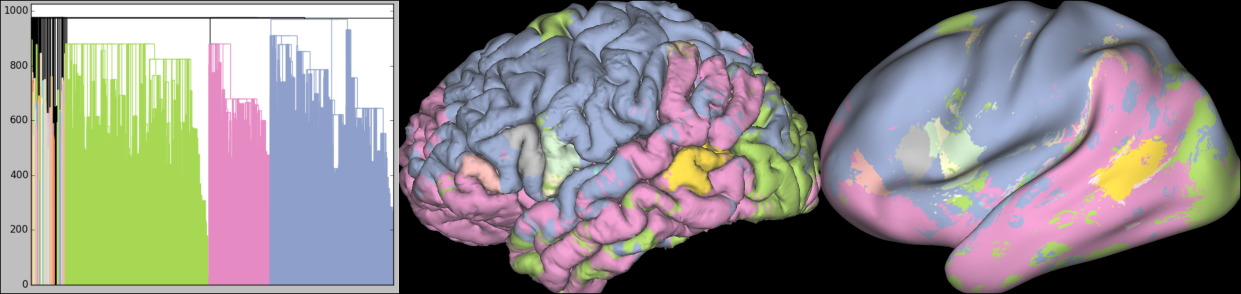
\includegraphics[width=\textwidth]{img/all_brain/logit_20000.png}
    \caption{M\'etodo Logit, veinte mil pasos de preprocesamiento}

\end{minipage} ~

\begin{minipage}[b]{\textwidth}
    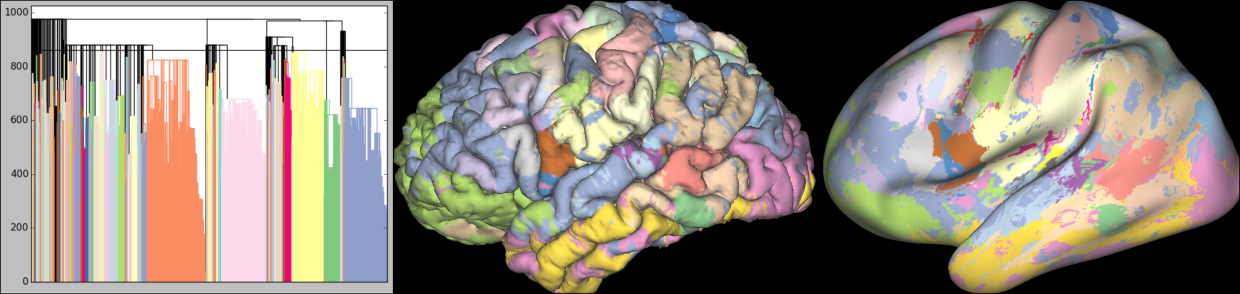
\includegraphics[width=\textwidth]{img/all_brain/logit_20000_deep0.png}
    \caption{M\'etodo Logit, veinte mil pasos de preprocesamiento, mayor 
             profundidad}
\end{minipage} ~

\begin{minipage}[b]{\textwidth}
    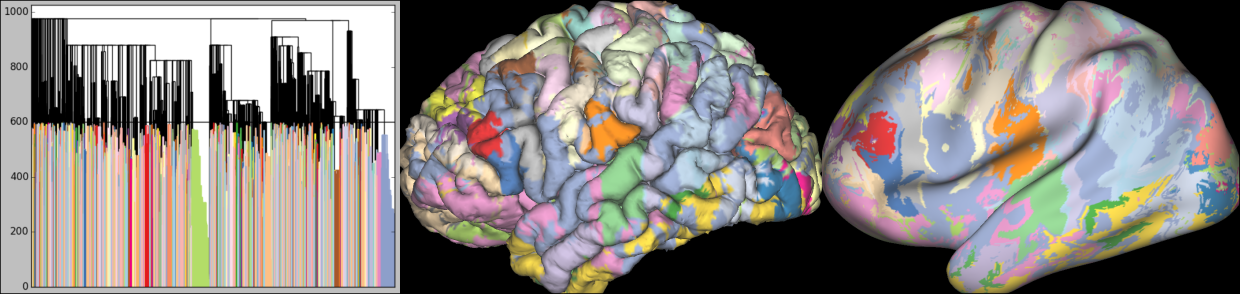
\includegraphics[width=\textwidth]{img/all_brain/logit_20000_deep1.png}
    \caption{M\'etodo Logit, veinte mil pasos de preprocesamiento, mayor 
             profundidad}
\end{minipage} ~


\end{figure}
